
\documentclass{article}

%% Packages for French writing
\usepackage[french]{babel}
\usepackage[utf8]{inputenc}
\usepackage[T1]{fontenc}
\usepackage{layout}

%% Packages for Math symbols
\usepackage[fleqn]{amsmath}
\usepackage{amssymb}
\usepackage{mathrsfs}

%% Packages for figures insertion
\usepackage{graphicx}
\usepackage{wrapfig}
\usepackage{framed}
\usepackage{float}

%% Package for document margin editing
\usepackage[top=2cm, bottom=2cm, left=2cm, right=2cm]{geometry}

%% Package for source code insertion
\usepackage{listings}
\usepackage{xcolor}
\definecolor{grey}{rgb}{0.97, 0.97, 0.97}
\definecolor{darkred}{rgb}{0.42, 0, 0}
\definecolor{darkblue}{rgb}{0, 0, 0.42}
\definecolor{darkgrey}{rgb}{0.22, 0.22, 0.82}
\definecolor{green}{HTML}{088A08}
\lstset{
  basicstyle=\small\sffamily\footnotesize,
  captionpos=b,
  numbers=left,
  numberstyle=\tiny,
  tabsize=4,
  frame=trBL,
  backgroundcolor=\color{grey},
  commentstyle=\color{green},
  keywordstyle=\color{darkblue}\bf,
  identifierstyle=\color{darkgrey},
  stringstyle=\color{darkred}
}

\setlength\parindent{0pt}
\setlength\parskip{3pt}
\title{Rapport de projet VLSI}
\author{Nicolas Phan, Kevin Mambu}
\date{pour le 26 Janvier 2018}
\begin{document}
\pagestyle{headings}
\maketitle
\tableofcontents
\newpage

%==================================================================================================
%=========================  Introduction  =========================================================
%==================================================================================================
\section{Introduction}

%----------------- Objectif -----------------------------------------------------------------------
\subsection{Objectif}

Le but de notre projet est de concevoir un processeur ARM, c'est à dire un processeur conforme
à l'architecture décrite dans la documentation ARM donnée en cahier des charges.

%----------------- Processus de developpement -----------------------------------------------------
\subsection{Processus de développement}

La conception de ce processeur se fera en quatre grandes étapes :

\begin{figure}[H]
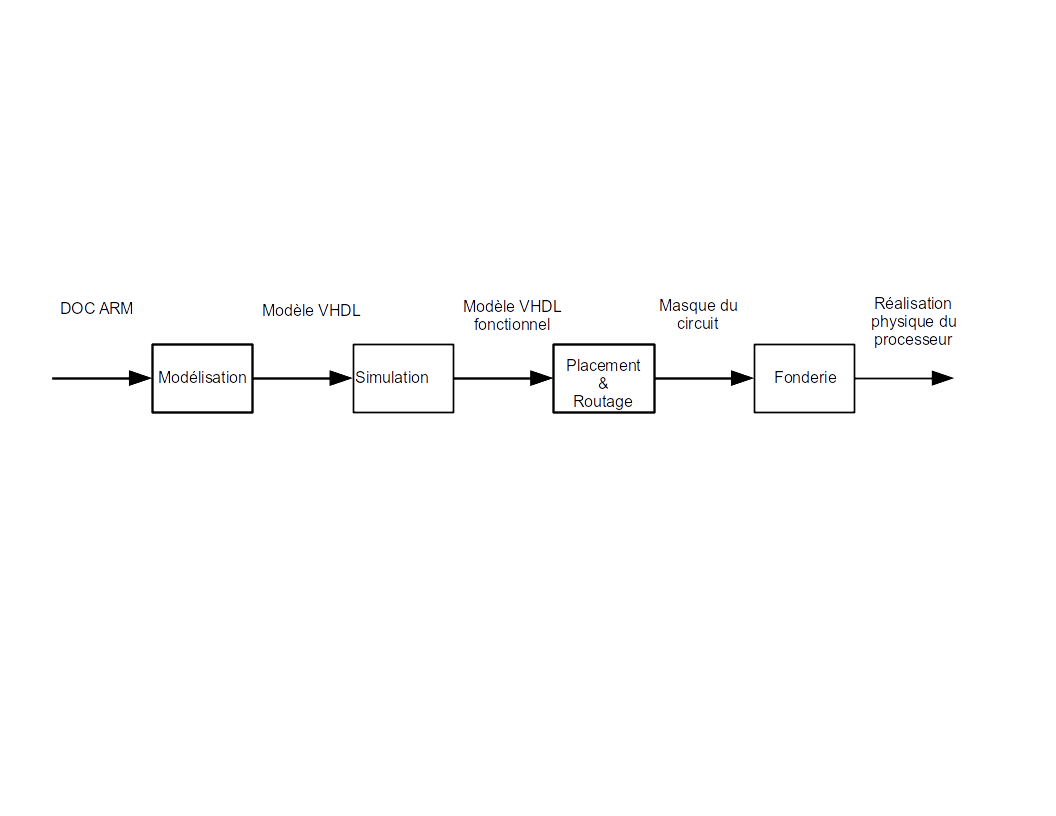
\includegraphics[width=0.75\textwidth]{pics/conception.png}
\centering
\caption{Schema-bloc des étapes de conception du processeur} 
\label{conception}
\end{figure}

\begin{enumerate}
\item \textbf{Modélisation}  : Cela consiste en la description d'un modèle du processeur,
                      la description peut avoir différents niveaux d'abstraction
                      du plus abstrait (description du comportement du circuit seulement)
                      au plus concret (schema des portes logiques du circuit)
                      \textit{Nous utiliserons le langage VHDL pour décrire notre modèle de processeur}
\item \textbf{Simulation}    : Il s'agit de simuler notre processeur.
                      \textit{Nous utiliserons le simulateur ghdl ainsi que des bancs de tests VHDL
                      et une plateforme de simulation d'exécution de programmes ASM et C}
\item \textbf{Placement, Routage} : Dans cette étape, nous passons d'un modèle VHDL du circuit à un
                          dessin du masque de notre processeur, prêt à être envoyé en fonderie.
                          \textit{Nous utiliserons les outils druc, cougar, lvx, tas et s2r pour cela}
\item \textbf{Fonderie} :          Cette étape est réalisée par un fondeur tiers.
\end{enumerate}

%==================================================================================================
%=========================  Modelisation  =========================================================
%==================================================================================================
\section{Modélisation}

%==================== Design general du processeur ================================================
\subsection{Design général du processeur}

Le processeur doit pouvoir exécuter toutes les instruction du jeu ARM avec le moins
de matériel possible, de plus, nous devrons concevoir un processeur pipeliné asynchrone.
La figure \ref{etages} illustre le découpage en étages de notre pipeline avec les opérations effectuées
par chaque étage pour chaque type d'instruction.
Les types d'instructions que nous étudierons seront les instructions de data processing (regops),
les instructions de branchement (branch), les transferts mémoires simples (trans) et multiples (mtrans).

\begin{figure}[H]
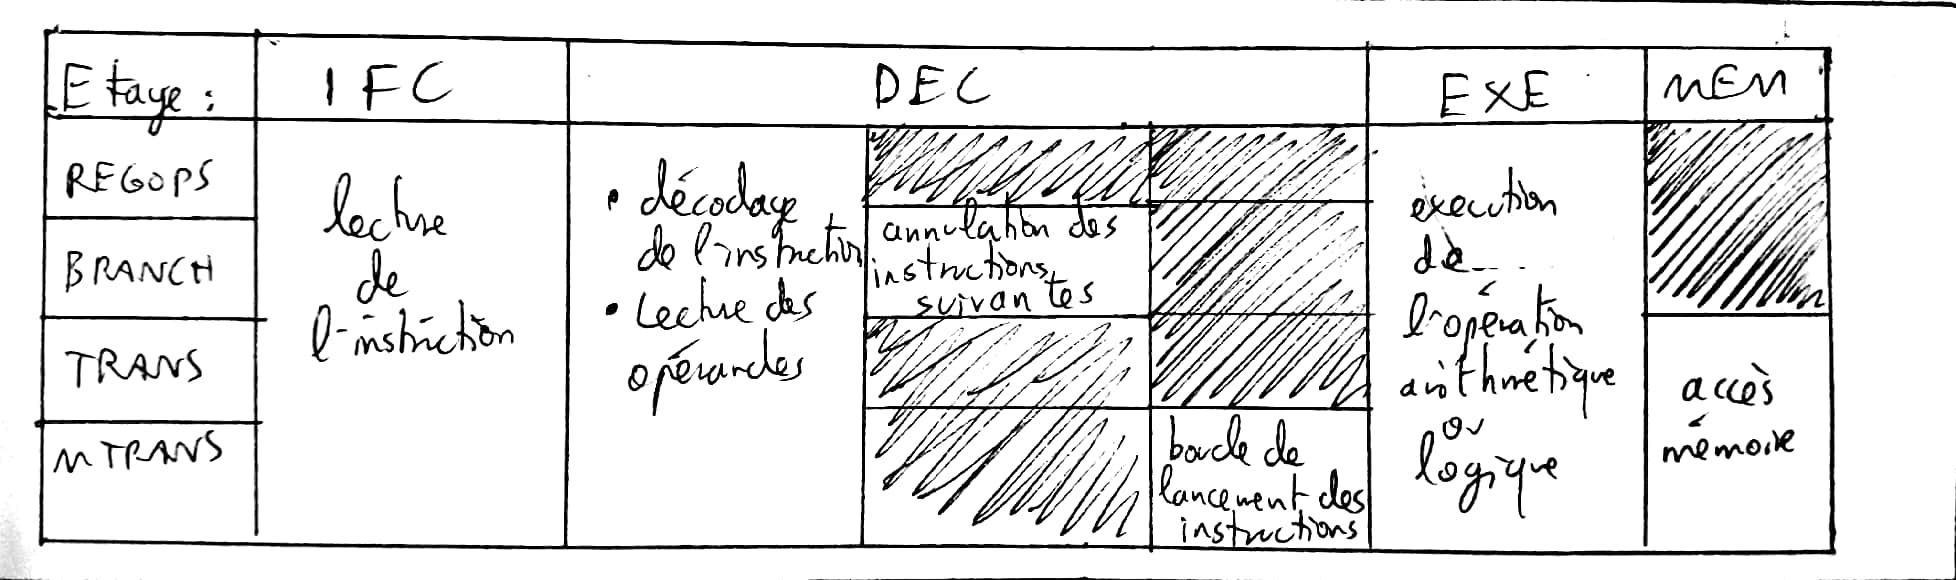
\includegraphics[width=0.75\textwidth]{pics/etages.png}
\centering
\caption{Découpage en étages du processeur}
\label{etages}
\end{figure}

%==================== Modelisation de l'etage EXE =================================================
\subsection{Modélisation de l'étage EXE}

\par
C'est à l'étage EXE que se feront les opérations de calcul lors de l'execution d'instructions,
cela comprend le calcul de l'adresse destination lors d'un branchement.
Pour concevoir cet étage, nous devons nous demander quelles sont tous les calculs possibles
que l'étage devra pouvoir réaliser.

\par
Les différents types d'instructions que nous avons sont les regops, les branch, les trans et mtrans,
or les branch, trans et mtrans n'ont besoin d'effectuer que des additions (pour le calcul d'adresses
mémoire) et les regops contiennent une instruction d'addition, donc si l'étage EXE peut effectuer
les calculs nécéssaires aux regops, a fortiori il couvre aussi les branch et transferts mémoire.
Cela réduit le problème au cas des regops.

\par
Il faut lister l'ensemble des calculs que EXE devra effectuer et les réécrire
de manière standardisée pour les décomposer en un sous-ensemble de calculs élémentaires.
Cela nous permettra de trouver une implémentation de EXE réduisant au maximum le matériel nécéssaire.

\begin{table}[H]
\centering
\begingroup
\setlength{\tabcolsep}{5pt}
\renewcommand{\arraystretch}{1.1}
\begin{tabular}{ | c | l | l | }
\hline
Instruction & Calcul demandé & Calcul standardisé  \\
\hline
\tt{AND}      & \tt{ op1 AND op2 }                 & \tt{ op1 AND op2 } \\
\hline
\tt{EOR}      & \tt{ op1 XOR op2 }                 & \tt{ op1 XOR op2 } \\
\hline
\tt{SUB}      & \tt{ op1 - op2 }                   & \tt{ op1 + $\overline{\tt{op2}}$ + 1 } \\
\hline
\tt{RSB}      & \tt{ op2 - op1 }                   & \tt{ $\overline{\tt{op1}}$ + op2 + 1} \\
\hline
\tt{ADD}      & \tt{ op1 + op2 }                   & \tt{ op1 + op2 } \\
\hline
\tt{ADC}      & \tt{ op1 + op2 + c }               & \tt{ op1 + op2 + c} \\
\hline
\tt{SBC}      & \tt{ op1 - op2 + c - 1 }           & \tt{ op1 + $\overline{\tt{op2}}$ + c} \\
\hline
\tt{RSC}      & \tt{ op2 - op1 + c - 1 }           & \tt{ $\overline{\tt{op1}}$ + op2 + c} \\
\hline
\tt{TST}      & \tt{ op1 AND op2 }                 & \tt{ op1 AND op2 } \\
\hline
\tt{TEQ}      & \tt{ op1 XOR op2 }                 & \tt{ op1 XOR op2 } \\
\hline
\tt{CMP}      & \tt{ op1 SUB op2 }                 & \tt{ op1 + $\overline{\tt{op2}}$ + 1 } \\
\hline
\tt{CMN}      & \tt{ op1 ADD op2 }                 & \tt{ op1 + op2 } \\
\hline
\tt{ORR}      & \tt{ op1 OR op2 }                  & \tt{ op1 OR op2 } \\
\hline
\tt{MOR}      & \tt{ op2 }                         & \tt{ 0 + op2 } \\
\hline
\tt{BIC}      & \tt{ op1 AND NOT op2 }             & \tt{ op1 AND $\overline{\tt{op2}}$ } \\
\hline
\tt{MVN}      & \tt{ NOT op2 }                     & \tt{ 0 + $\overline{\tt{op2}}$ } \\
\hline
\end{tabular}
\endgroup
\caption{Standardisation des calculs demandés par les regops}
\label{standard}
\end{table}

On peut voir sur la Table \ref{standard} que l'ensemble des calculs demandés se décompose
en calculs élémentaires suivants :
\begin{itemize}
  \item ADD, AND, OR, XOR
  \item Inversion des entrées au préalable
  \item Ajout d'un 1 pour l'addition (retenue en entrée)
\end{itemize}

De plus, le jeu d'instruction ARM spécife que l'opérande 1 peut subir un décalage
parmi 5 types (lsl, lsr, asr, ror, rrx) et qu'à chaque opération, les flags de sortie
doivent être calculés, on a donc :
\begin{itemize}
  \item Décalage de l'opérande 1
  \item Calcul des flags de sortie
\end{itemize}

Avec tous ces éléments, nous aboutissons au schema Figure \ref{exe} pour EXE.

\begin{figure}[H]
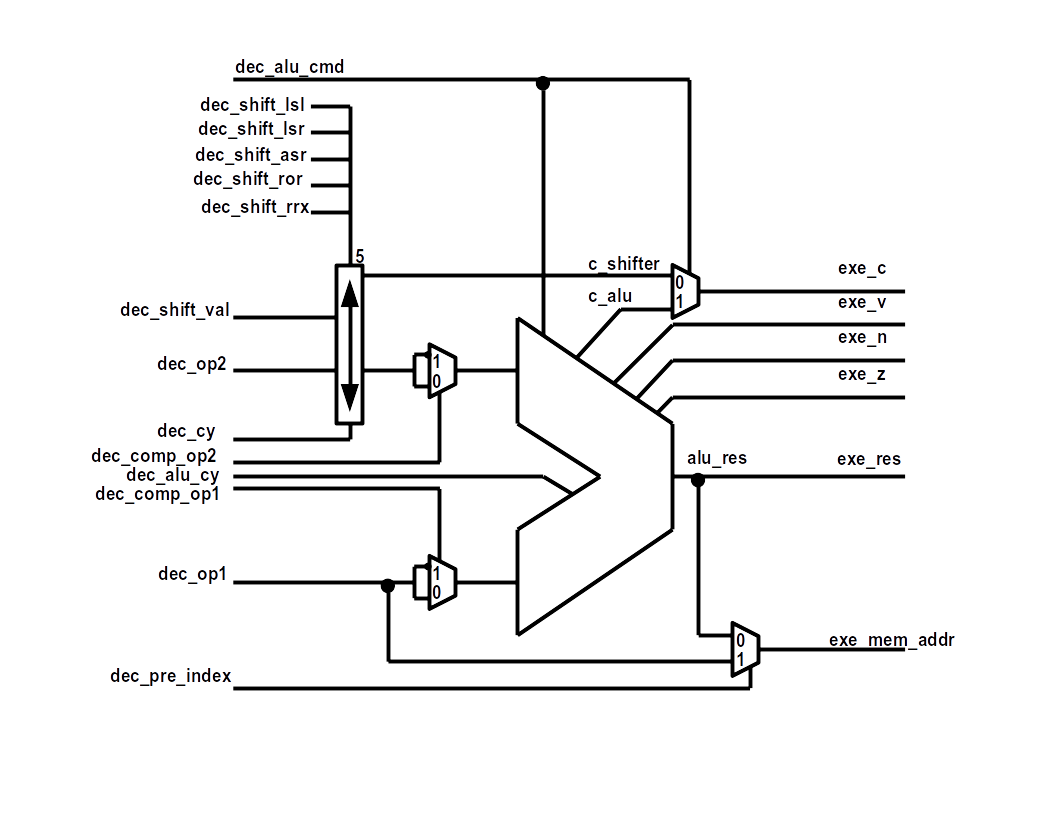
\includegraphics[width=0.75\textwidth]{pics/exe.png}
\centering
\caption{Schema de l'étage EXE}
\label{exe}
\end{figure}

\subsubsection{Modélisation de l'ALU}

L'ALU doit pouvoir effectuer les opérations ADD, AND, OR et XOR sur deux entrées de 32bits,
et pour l'addition elle doit pouvoir prendre en compte une retenue en entrée et en sortie.

Notre implémentation est celle en Figure \ref{alu} : L'ALU effectue de toutes manières les
4 opérations sur ses entrées, mais ne prend que le résultat de l'opération qui nous intéresse.

Pour le calcul des flags, le bloc "=0" effectue un simple AND entre tous les bits du résultat,
le bloc "<0" vérifie si le MSB est égal à 1, on remarque que par la manière dont est construit
le système de nombres signés, la condition "<0" est très simple à vérifier. Puis pour le bloc "overflow",
on prend le 33ème bit du résultat de l'addition, il y a overflow s'il n'est pas nul (le résultat va au-delà
du range des 32 bits).

\begin{figure}[H]
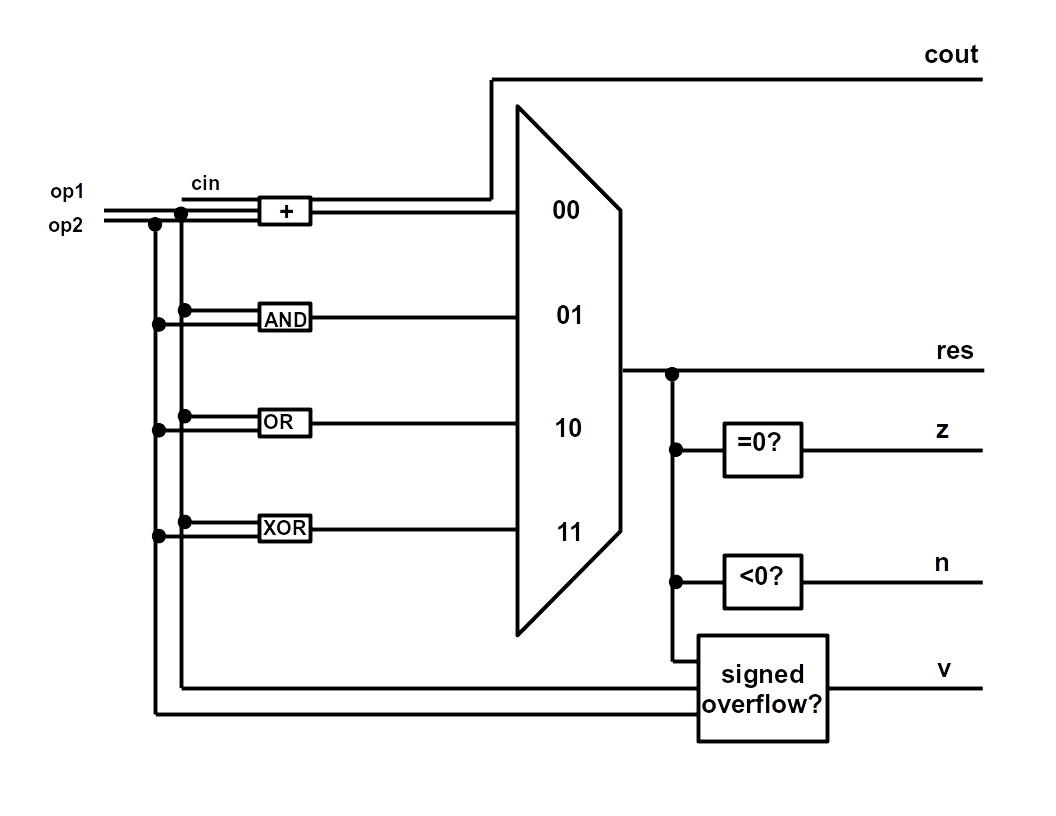
\includegraphics[width=0.75\textwidth]{pics/alu.png}
\centering
\caption{Schema de l'ALU}
\label{alu}
\end{figure}

\subsubsection{Modélisation du Shifter}

Tout comme l'ALU peut effectuer différentes opérations, le shifter peut effectuer différents
types de décalages (LSL, LSR, ASR, ROR, RRX) donc de la même manière, notre implémentation
du shifter en Figure \ref{shifter} effectue tous les types de décalages possibles et choisit
le résultat qui nous intéresse.

\begin{figure}[H]
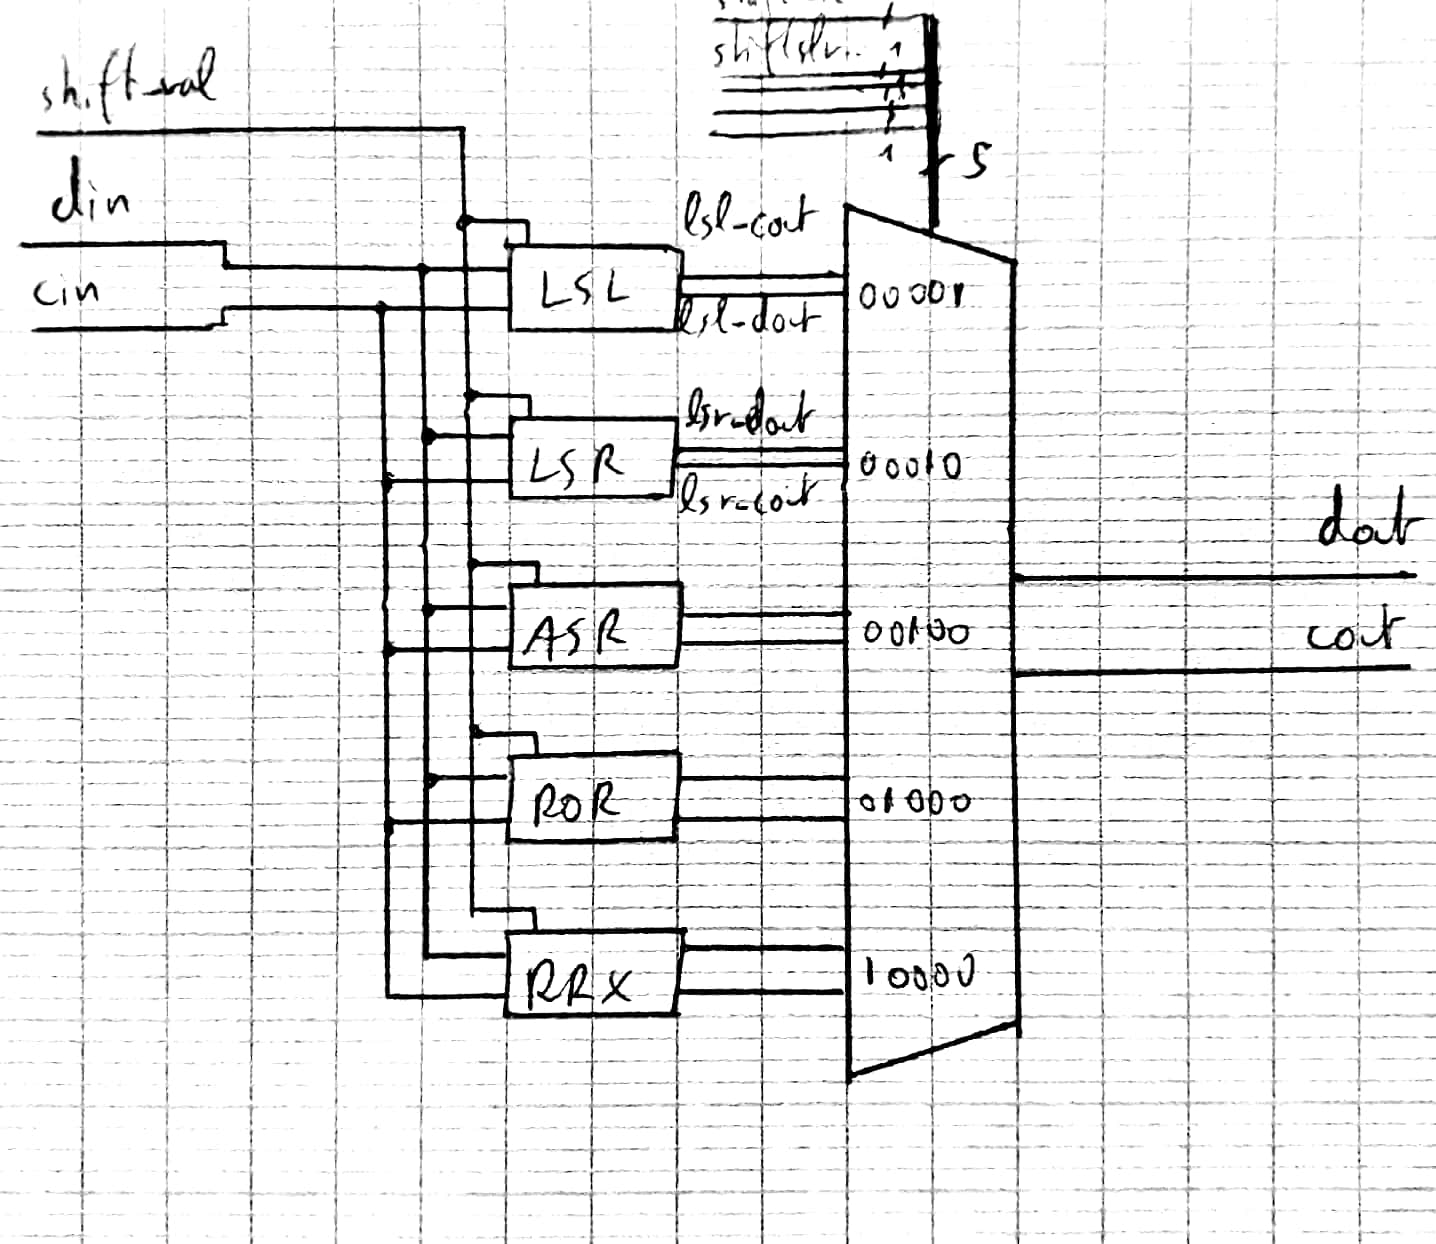
\includegraphics[width=0.75\textwidth]{pics/shifter.png}
\centering
\caption{Schema du Shifter}
\label{shifter}
\end{figure}

Ensuite pour réaliser l'opération LSL, en Figure \ref{shifter_lsl},
on observe chaque bit du \texttt{shift\_value} :
si le bit $n$ est à \texttt{1}, alors l'opérande subit un décalage de $2^n$.
Le décalage total subi par l'opérande source est donc de :

\begin{eqnarray*}
  \sum_{\substack{k \in [[0, 31]] \\ \texttt{shift\_value(k)} = 1}} 2^k &= \texttt{shift\_value}
\end{eqnarray*}

La même logique est utilisée pour implémenter les autres types de décalages.

\begin{figure}[H]
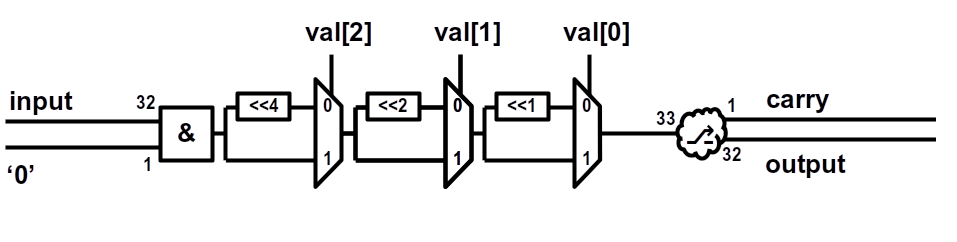
\includegraphics[width=0.75\textwidth]{pics/shifter_lsl.png}
\centering
\caption{Schema de la partie LSL du Shifter}
\label{shifter_lsl}
\end{figure}



\subsubsection{Ajouts sur EXE}

\textbf{Le flag C}

D'après la doc ARM, le flag C en sortie d'une opération peut être la retenur en sortie d'addition
pour les opérations arithmétiques ou en sortie de shift pour les opérations logiques.
Puis pour savoir si l'opération en cours est arithmérique ou logique, il suffit de voir si
l'ALU réalise une addition ou autre chose.

\textbf{La pre/post indexation}

Lors d'un accès mémoire, le jeu ARM offre la possibilité de choisisr si l'adresse prise en compte
pour un accès mémoire est l'adresse de base ou l'addresse base + offset.
Dans EXE, cela équivaut à choisir entre l'opérande 2 et le résultat en sortie d'ALU,
cela mène au schema en Figure \ref{exe2}.

\begin{figure}[H]
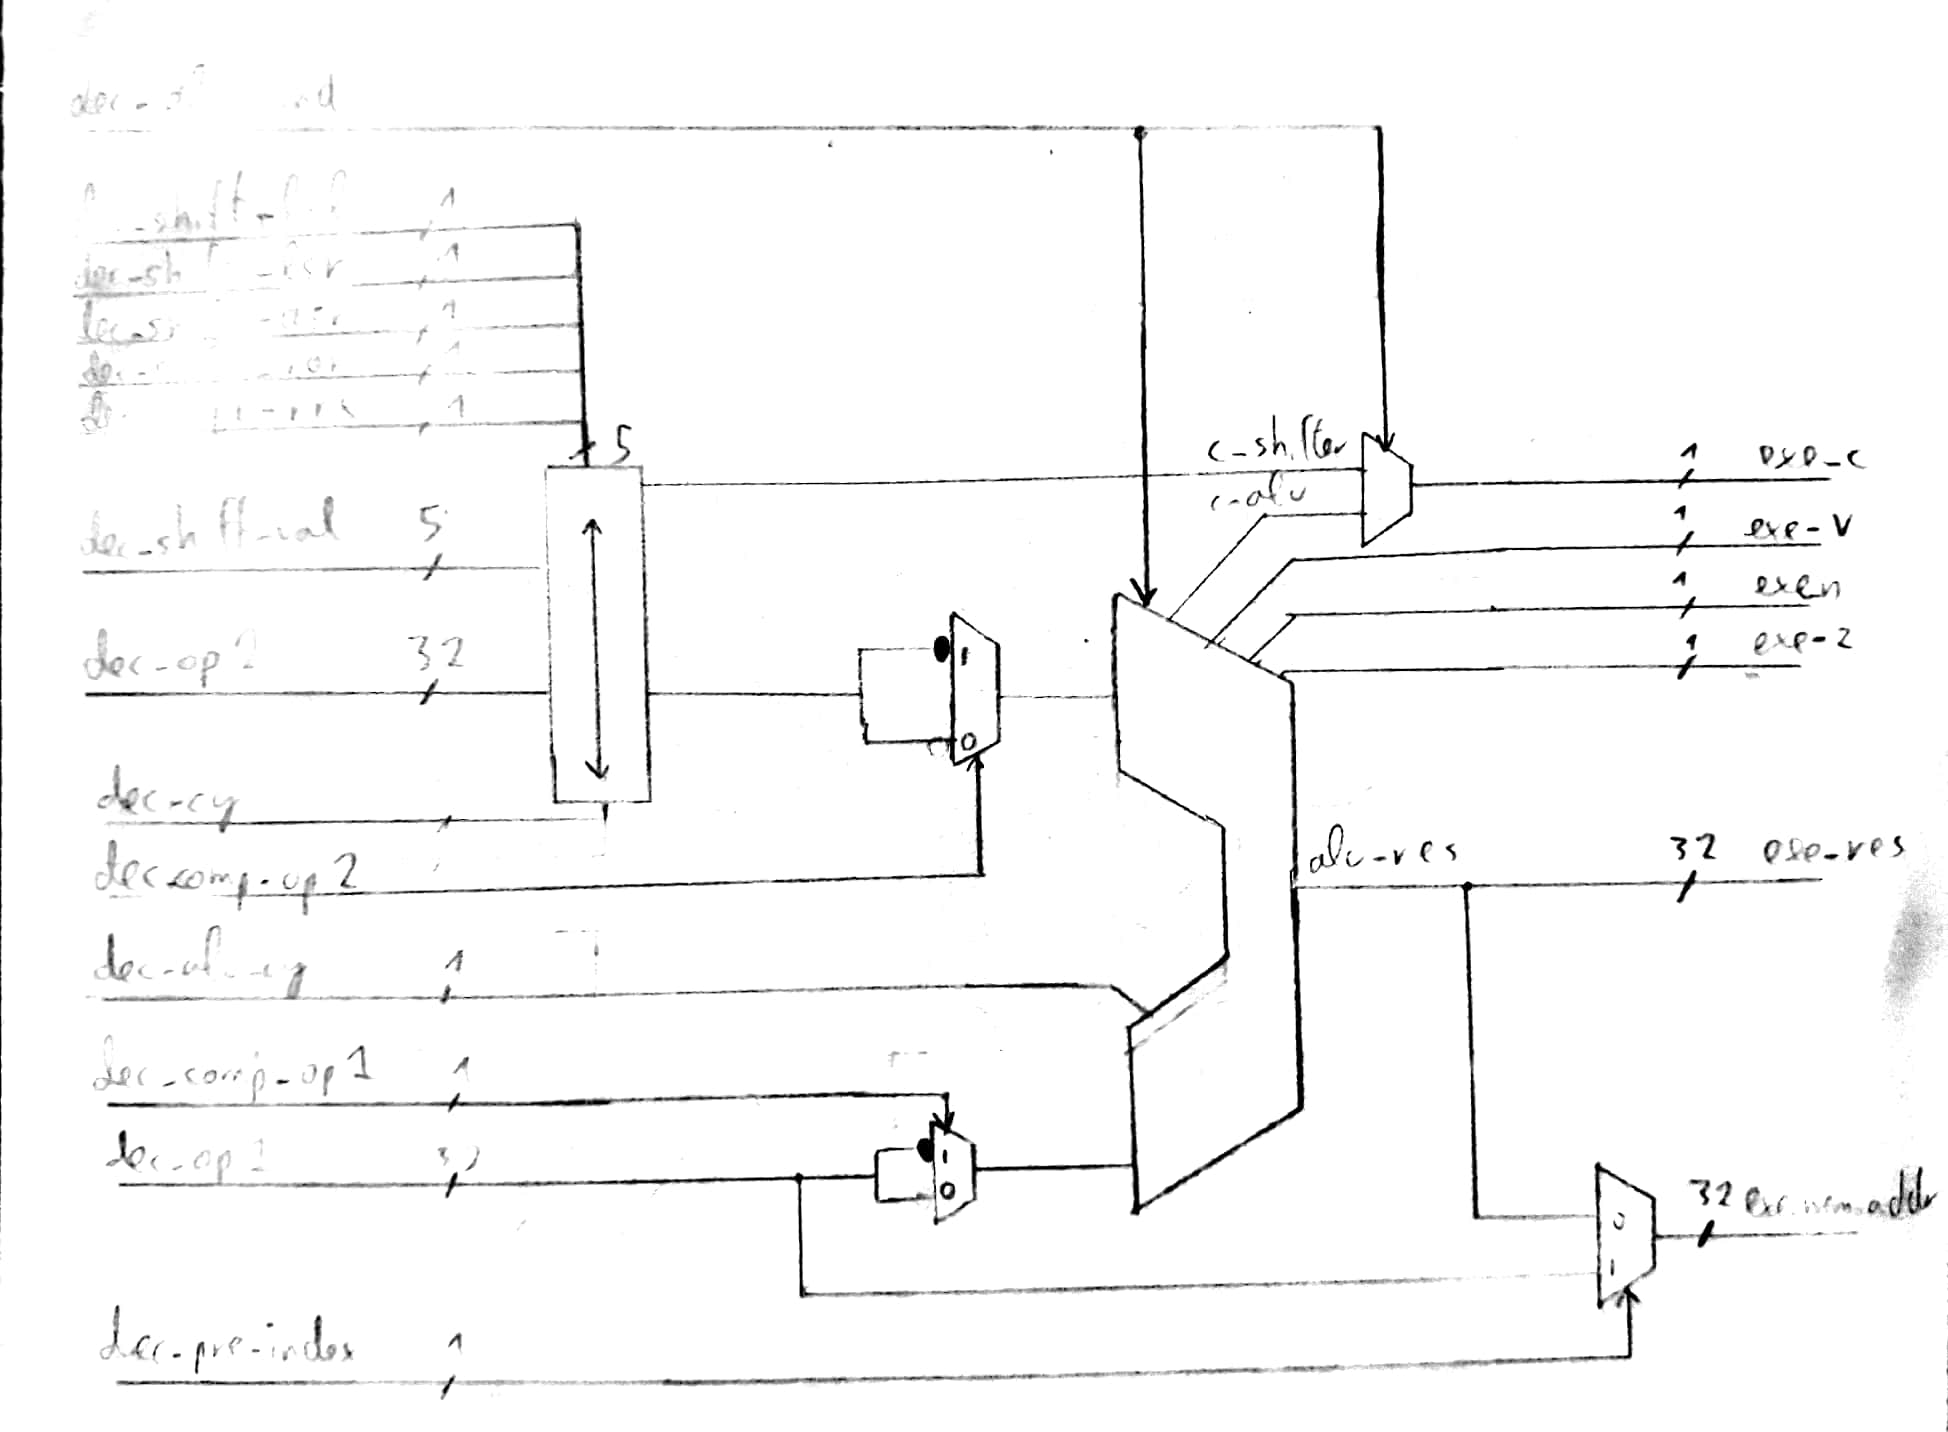
\includegraphics[width=0.75\textwidth]{pics/exe2.png}
\centering
\caption{Schema amélioré de EXE}
\label{exe2}
\end{figure}

%==================== Modelisation de l'etage DEC =================================================
\section{Modélisation de l'étage DECOD}

Pour chaque instruction, hormis quelques spécificités dues aux branchements
et transferts multiples, DECOD doit faire 5 choses :
\begin{enumerate}
  \item Envoyer l'adresse de l'instruction (valeur de PC) vers IFC.
  \item Récupérer l'instruction de IFC.
  \item Décoder l'instruction (quel opération effectuer, quelles opérandes utiliser)
  \item Vérifier si la condition d'exécution est remplie (exécution conditionnelle)
  \item Lire les opérandes à utiliser sur le banc de registres.
  \item Envoyer les opérandes lues et le type d'opération à effectuer vers EXE.
  \item Passer à l'instruction suivante (incrémenter PC)
\end{enumerate}

Dans un premier temps, nous modéliserons le comportement général de DECOD,
puis nous apporterons des amélioration au fur et à mesure pour implémenter les branchements,
les branchements avec link puis les transferts multiples. Nous avons donc choisi une approche
"instruction par instruction" pour la modélisation de DECOD.

Le premier type d'instruction à implémenter sont les regops, elles ne font rien de spécial
à DECOD donc c'est adapté de commence par elles pour implémenter le comportement général de DECOD.
Dans DECOD nous placerons le bang de registres (REG), nous verrons donc un par un les choses
à implémenter dans DECOD et dans REG.

\subsection{Envoi du PC vers IFC}

Nous plaçons dans REG la sortie \texttt{reg\_pc} qui donne à DEC la valeur de PC à chaque instant,
puis DEC transmet cette valeur à IFC sur la sortie \texttt{dec\_pc} via une FIFO (dec2if).

\begin{figure}[H]
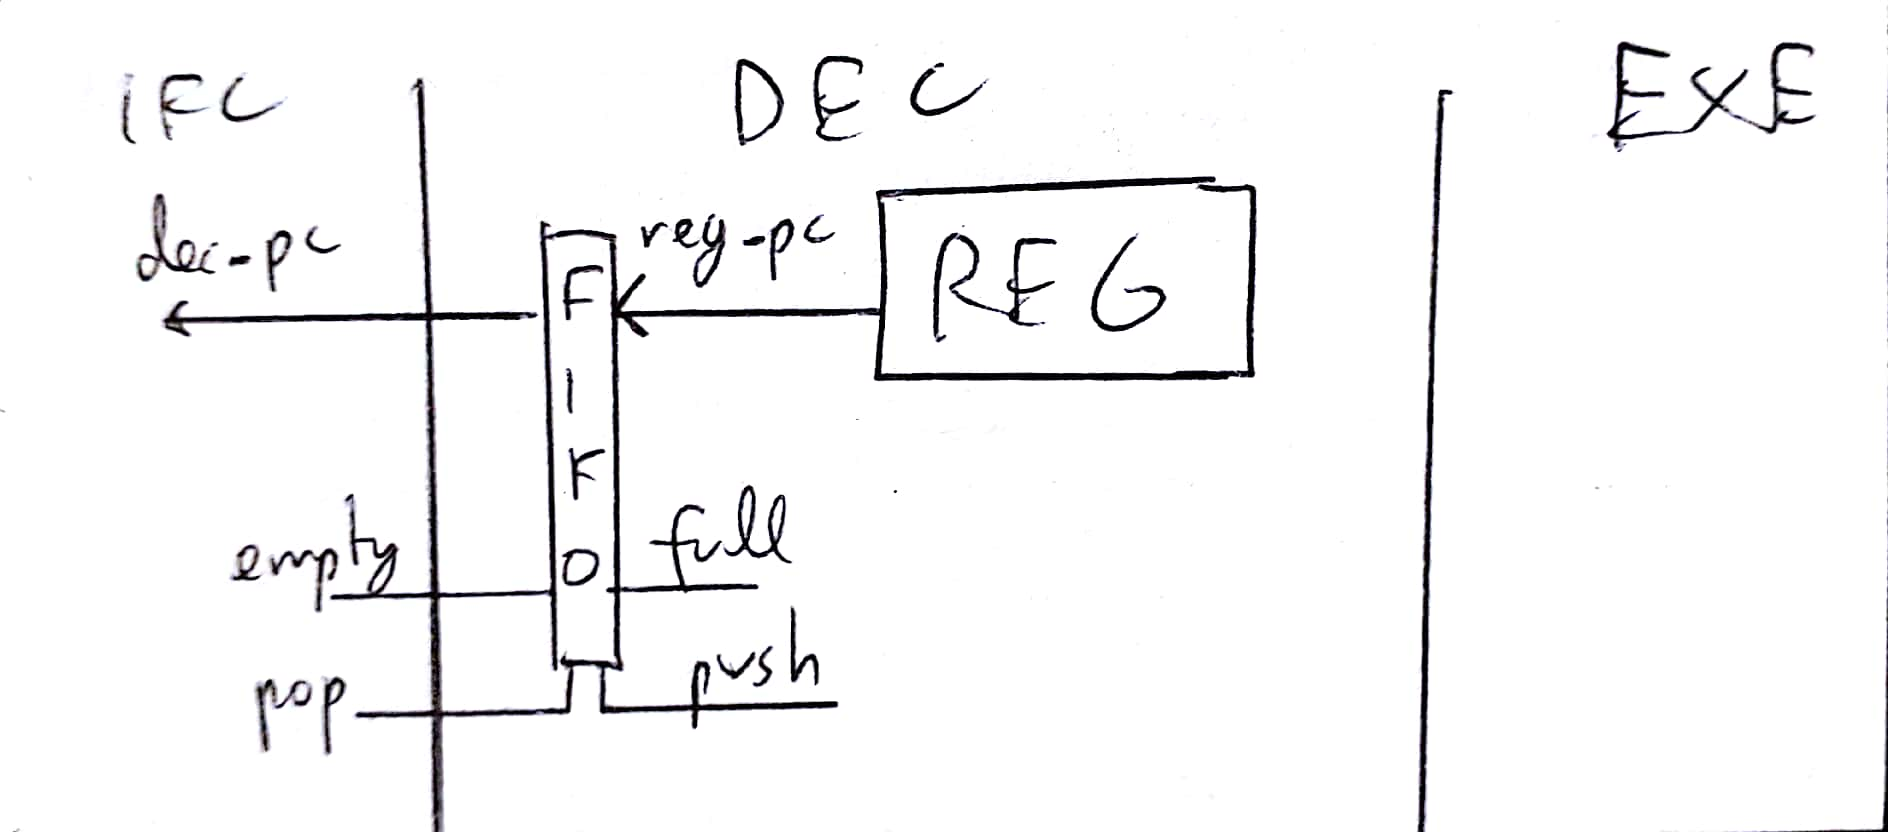
\includegraphics[width=0.75\textwidth]{pics/dec1.png}
\centering
\caption{Schema temporaire de DECOD}
\label{dec1}
\end{figure}

\subsection{Récupération de l'instruction depuis IFC}

Il y a encore communication entre deux étages, donc nous avons encore une FIFO (if2dec)
mais comme la convention veut que la FIFO soit à l'étage émetteur, elle sera dans IFC,
donc dans DEC nous récupérons simplement l'instruction via une entrée \texttt{if\_ir[32bits]}.

\begin{figure}[H]
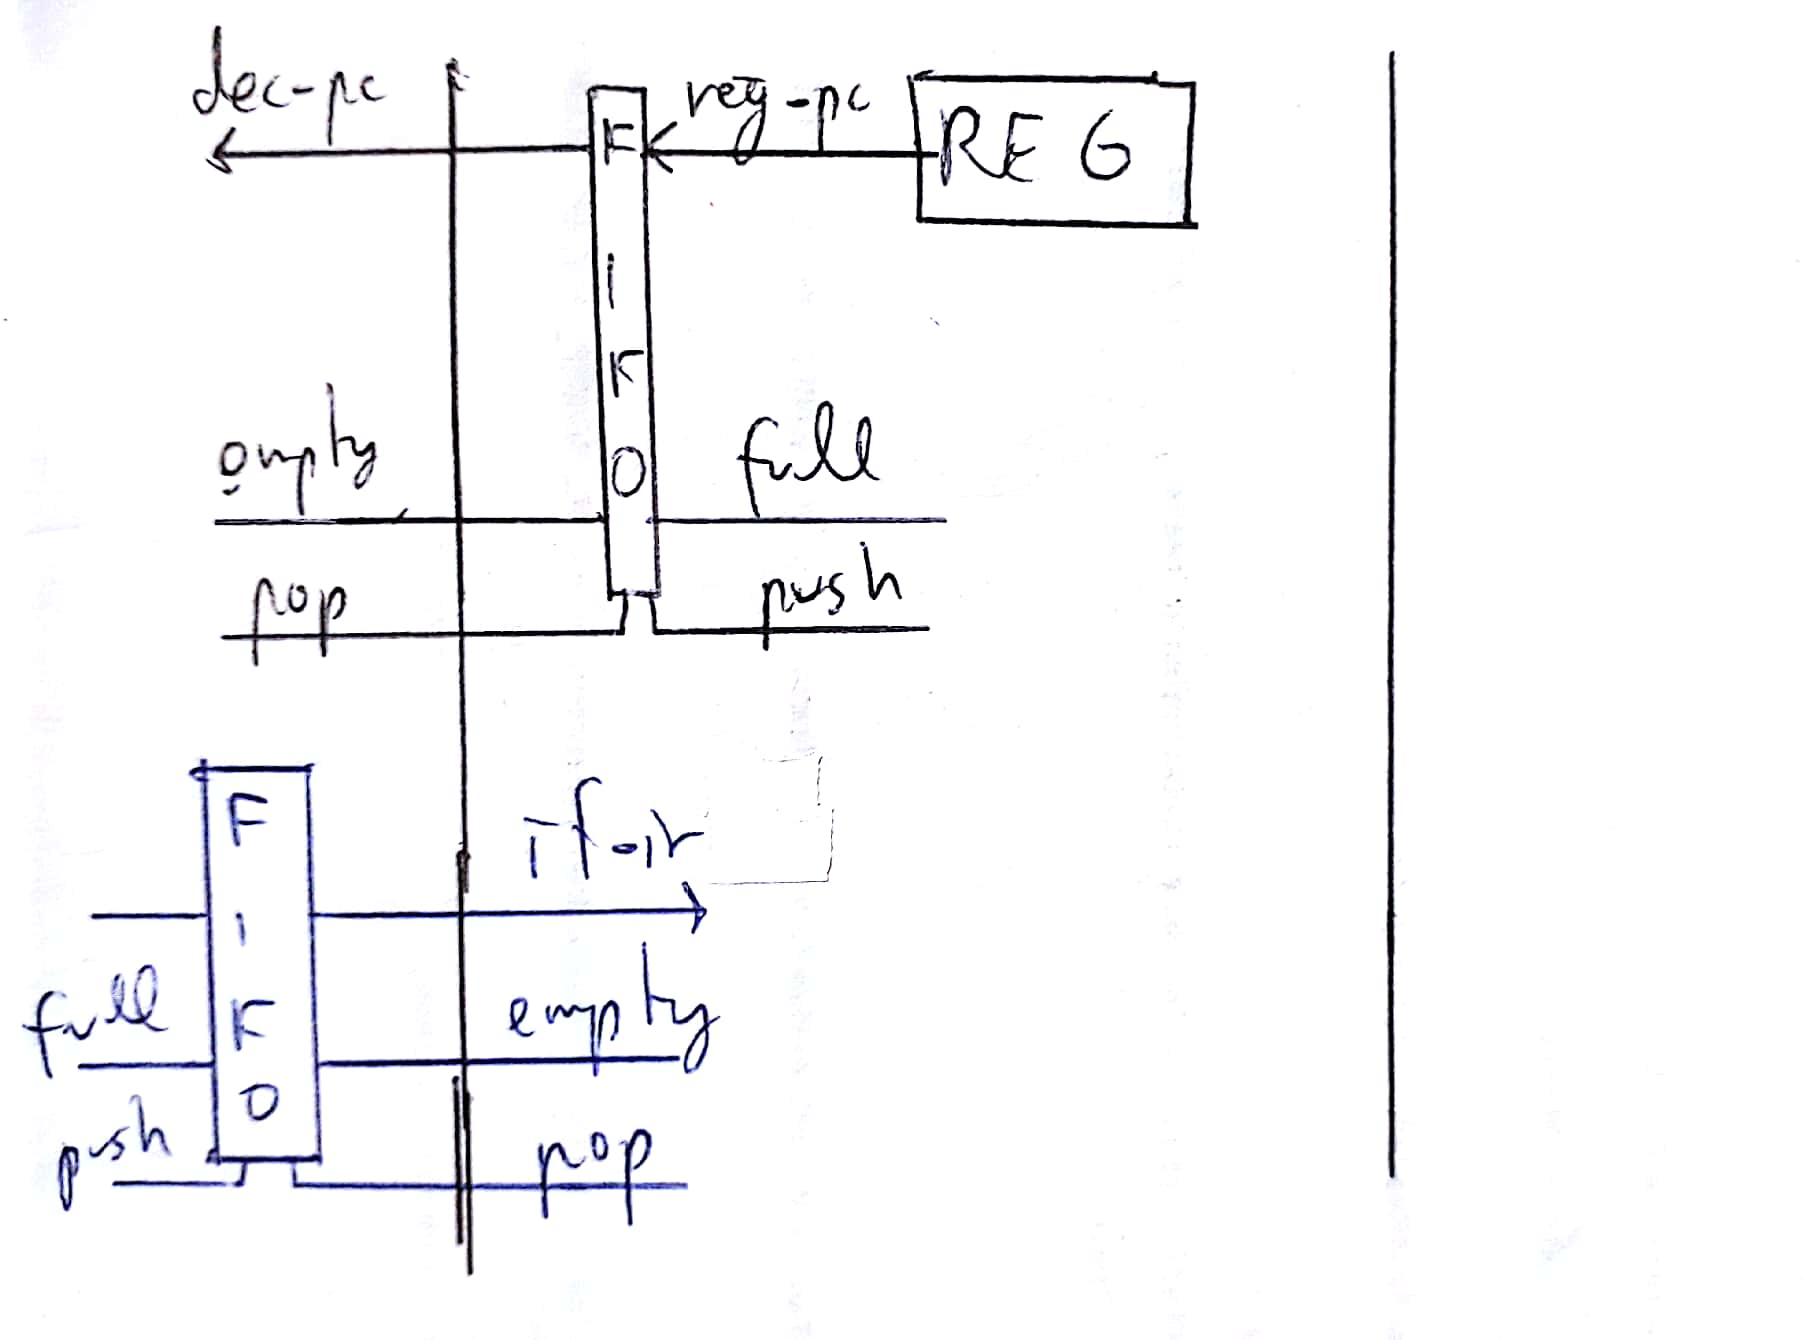
\includegraphics[width=0.75\textwidth]{pics/dec2.png}
\centering
\caption{Schema temporaire de DECOD}
\label{dec2}
\end{figure}


\subsection{Décodage de l'instruction}

\subsubsection{Decodage du type d'instruction}

Il s'agit ici de lire, à partir des 32 bits de \texttt{if\_ir}, quelle opération
doit être effectuée et sur quelles opérandes.

La première chose à décoder est le type d'instruction. Selon le détail du format des
instructions en Figure ..., si on ne considère que les instruction :
\begin{enumerate}
  \item Data processing
  \item Multiply
  \item Single Data Swap
  \item Single Data Transfert
  \item Block Data Transfert
  \item Branch
\end{enumerate}

Le premier critère est que les bits 27 à 25 valent :
\begin{enumerate}
  \item 00X    pour les regops, les multiply et swap
  \item 01X    pour les single data transfert
  \item 100    pour les multiple transferts
  \item 101    pour les branch
\end{enumerate}

Ensuite, pour distinguer les regops, multiply et swap, le deuxième critère est que :
\begin{enumerate}
  \item Pour les mult, les bits 25 à 23 valent 000 et les bits 7 à 4 valent 1001
  \item Pour les swap, les bits 25 à 23 valent 101 et les bits 7 à 4 valent 1001
\end{enumerate}
On pourrait penser a priori que les regops pourraient, dans leur opérande 2,
avoir leurs bits 7 à 4 égaux à 1001 mais dans le détail de l'opérande 2 et du shift,
on observe que si le bit 4 vaut 1, le bit 7 vaut forcément 0 donc cette combinaison est impossible,
il n'y a donc pas de conflit potentiel.

%code : les xxx_t
\lstinputlisting[language=vhdl, firstline=560, lastline=579]{decod.vhdl}

\subsubsection{Decodage de l'instruction}

Maintenant qu'on connait de type d'instruction, il faut déterminer à quelle instruction
on a affaire précisément.

Pour les regops, c'est immédiat : les bits 24 à 21 de \texttt{if\_ir} donnent directement l'opcode,
d'ou. (Pour les trans (Single Data Transfert), il suffit de lire les bits 20 et 22 qui donnent
respectivement le sens d'accès (lecture/écriture) et la taille de la données accédée (mot/octet)).

%code : les xxx_i
\lstinputlisting[language=vhdl, firstline=581, lastline=615]{decod.vhdl}

La figure \ref{dec3} résume ce qu'il a dans DECOD pour l'instant.

\begin{figure}[H]
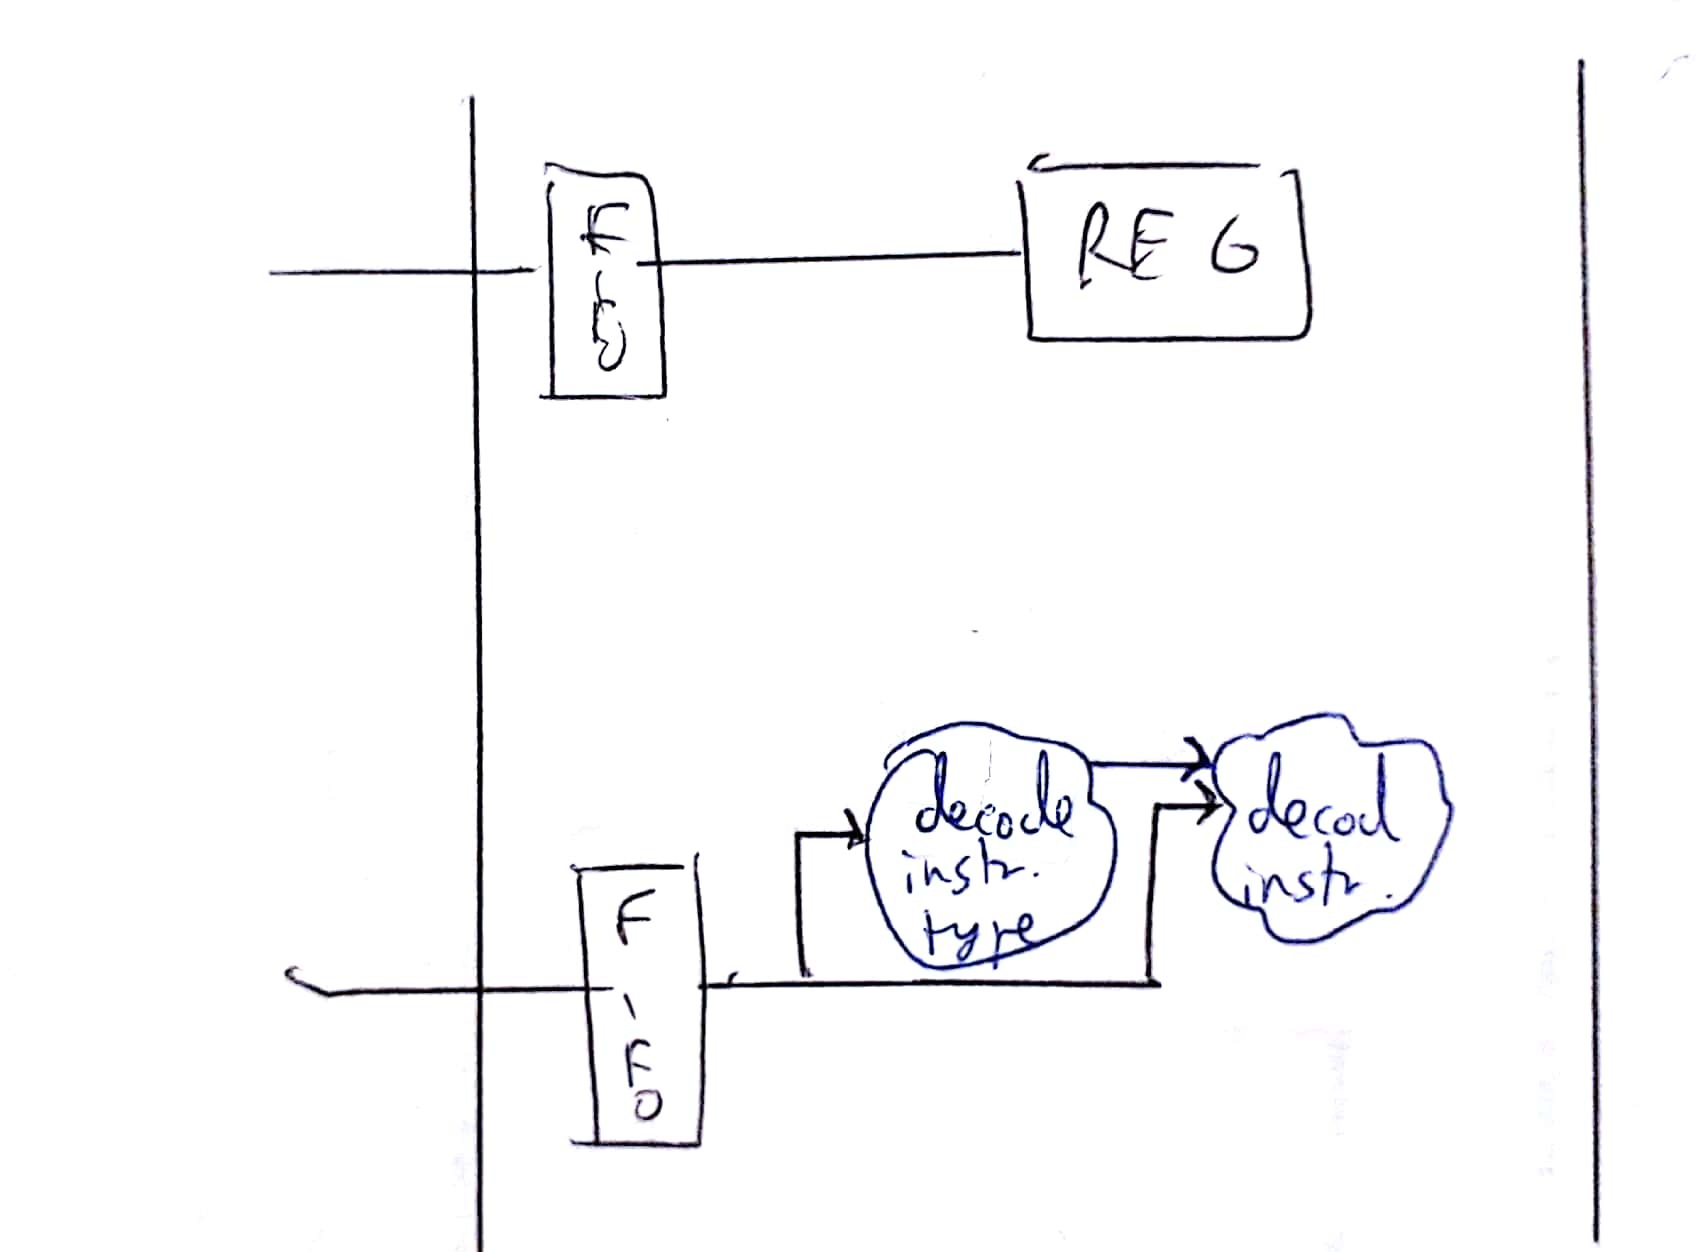
\includegraphics[width=0.75\textwidth]{pics/dec3.png}
\centering
\caption{Schema temporaire de DECOD}
\label{dec3}
\end{figure}


\subsection{Lecture des opérandes}

L'exécution d'une instruction nécéssite de récupérer la valeur de certains registres pour
effectuer une opération dessus (ce sera EXE qui la fera). DECOD doit se charger
de lire les registres nécéssaires depuis le banc de registres pour fournir leurs valeurs à EXE.

Pour cela, nous placerons 3 ports de lecture dans REG (3 car les instruction ont besoin de
connaître au maximum les valeurs de 3 registres). La lecture se fera au sein d'un même cycle d'horloge
car tout ce que fait DECOD doit se faire en un cycle.

Ensuite, DECOD doit déterminer quels registres lire à chaque fois.
Dans la documentation ARM, les registres à lire potentiellement sont Rd, Rn, Rm et Rs,
nous assignerons:
\begin{enumerate}
  \item Le port de lecture 1 de REG     à Rn,
  \item Le port 2 à Rm
  \item Le port 3 à Rd et Rs
\end{enumerate}
Aucune instruction ne lit Rd et Rs en même temps, donc il n'y aura pas de conflit sur le port 3.
Puis le numéro des registres Rn, Rm, Rd et Rs est données dans \texttt{if\_ir}, encore selon la doc ARM :
\begin{enumerate}
  \item Rd est donné dans les bits 15 à 12 (sauf pour le mult ou c'est de 19 à 15)
  \item Rn -> \texttt{if\_ir(19:16)} sauf pour les mult où c'est \texttt{if\_ir(15:12)}
  \item Rm -> \texttt{if\_ir(3:0)}
  \item Rs -> \texttt{if\_ir(11:8)}
\end{enumerate}
Il suffit de récupérer ces champs et de les donner en adresse à REG pour obtenir nos valeurs de registres :

%code : les radr
\lstinputlisting[language=vhdl, firstline=759, lastline=770]{decod.vhdl}

\subsection{Envoi de l'opération à EXE}

Une fois les opérandes lues, il s'agit de les envoyer vers EXE ainsi que les détails
sur l'opération à effectuer, c'est à dire les signaux :
\begin{enumerate}
  \item \texttt{alu\_dest}
  \item \texttt{op1}
  \item \texttt{op2}
  \item \texttt{alu\_cmd}
  \item \texttt{alu\_cy}
  \item \texttt{comp\_op1}
  \item \texttt{comp\_op2}
  \item \texttt{shift\_lsl}
  \item \texttt{shift\_lsr}
  \item \texttt{shift\_asr}
  \item \texttt{shift\_ror}
  \item \texttt{shift\_rrx}
  \item \texttt{shift\_val}
\end{enumerate}

Nous nous concentrerons sur le cas des regops.

\texttt{alu\_dest} sera Rd, c'est à dire \texttt{if\_ir(15:12)}.
op1 sera la valeur de Rn, (port 1 de REG)
op2 sera soit la valeur de Rm (port 2 de REG), soit un immediat (\texttt{if\_ir(7 downto 0)} zero-extended)

Quant à \texttt{alu\_cmd}, \texttt{alu\_cy}, \texttt{comp\_op1} et \texttt{comp\_op2},
leur valeur dépend de l'instruction en question,
le Tableau \ref{regops-exe} détaille leurs valeurs.

\begin{table}[H]
\centering
\begingroup
\setlength{\tabcolsep}{5pt}
\renewcommand{\arraystretch}{1.1}
\begin{tabular}{ | c | l | c | c | c | c | }
\hline
Instruction & Calcul standardisé  & alu\_cmd & comp\_op1 & comp\_op2 & carry \\
\hline
\tt{AND}    &  \tt{ op1 AND op2 } &                             AND & 0 & 0 & 0 \\
\hline
\tt{EOR}    &  \tt{ op1 XOR op2 } &                             XOR & 0 & 0 & 0 \\
\hline
\tt{SUB}    &  \tt{ op1 + $\overline{\tt{op2}}$ + 1 } &           + & 0 & 1 & 1 \\
\hline
\tt{RSB}    &  \tt{ $\overline{\tt{op1}}$ + op2 + 1} &            + & 1 & 0 & 1 \\
\hline
\tt{ADD}    &  \tt{ op1 + op2 } &                                 + & 0 & 0 & 0 \\
\hline
\tt{ADC}    &  \tt{ op1 + op2 + c} &                              + & 0 & 0 & c \\
\hline
\tt{SBC}    &  \tt{ op1 + $\overline{\tt{op2}}$ + c} &            + & 0 & 1 & c \\
\hline
\tt{RSC}    &  \tt{ $\overline{\tt{op1}}$ + op2 + c} &            + & 1 & 0 & c \\
\hline
\tt{TST}    &  \tt{ op1 AND op2 } &                             AND & 0 & 0 & 0 \\
\hline
\tt{TEQ}    &  \tt{ op1 XOR op2 } &                             XOR & 0 & 0 & 0 \\
\hline
\tt{CMP}    &  \tt{ op1 + $\overline{\tt{op2}}$ + 1 } &           + & 0 & 1 & 1 \\
\hline
\tt{CMN}    &  \tt{ op1 + op2 } &                                 + & 0 & 0 & 0 \\
\hline
\tt{ORR}    &  \tt{ op1 OR op2 } &                               OR & 0 & 0 & 0 \\
\hline
\tt{MOR}    &  \tt{ 0 + op2 } &                                  OR & 0 & 0 & 0 \\
\hline
\tt{BIC}    &  \tt{ op1 AND $\overline{\tt{op2}}$ } &           AND & 0 & 1 & 0 \\
\hline
\tt{MVN}    &  \tt{ 0 + $\overline{\tt{op2}}$ } &                OR & 0 & 1 & 0 \\
\hline
\end{tabular}
\endgroup
\caption{Standardisation des calculs demandés par les regops}
\label{regops-exe}
\end{table}


Enfin, il faut spécifier quel décalage appliquer à l'opérande 2.
Le type de décalage est donné par \texttt{if\_ir(6:5)} mais dans le cas des rotations,
il faut distinguer ROR et RRX dans le cas \texttt{if\_ir(6:5)} = \texttt{"11"} :
On a un ROR si l'opérande 2 est un immédiat ou si c'est un register mais que le shift amount n'est pas nul.



%==================================================================================================
%=========================  End of the Document  ==================================================
%==================================================================================================

\end{document}
